
\PassOptionsToPackage{colorlinks,linkcolor={blue},citecolor={blue},urlcolor={blue},breaklinks=true,final}{hyperref}
\PassOptionsToPackage{dvipsnames}{xcolor}
\documentclass[xcolor={dvipsnames,svgnames},aspectratio=169]{beamer}

\usepackage{fontawesome5}
\usepackage{booktabs} % For better table formatting
\usepackage{listings}
\usepackage{tabularx}


\lstset{
  tabsize = 4, %% set tab space width
  showstringspaces = false, %% prevent space marking in strings, string is defined as the text that is generally printed directly to the console
  numbers = left, %% display line numbers on the left
  commentstyle = \color{purple!60}, %% set comment color
  keywordstyle = \color{blue}, %% set keyword color
  stringstyle = \color{red}, %% set string color
  rulecolor = \color{black}, %% set frame color to avoid being affected by text color
  basicstyle = \small \ttfamily , %% set listing font and size
  breaklines = true, %% enable line breaking
  numberstyle = \tiny,
}

\title{Concurrent Programming}
\subtitle{Week 14 (Lecture 6) : \textbf{Queues, tasks and executors}}
\author{Stelios Tsampas}
\institute{
  \faEnvelope \; stelios@imada.sdu.dk
  \qquad
  \faGlobe \;
  \href{https://www.steliostsampas.com}{https://www.steliostsampas.com}
  \\\\\
  \faGithub \; stelios-tau/cp-2025
  \qquad\;\;
    \faDiscord \; cp-2025
}
\date{\today}

\titlegraphic{\includegraphics[height=0.6cm,keepaspectratio]{../media/sdu-black.eps}}

\usetheme[block=fill]{metropolis}


%\usepackage{pres-common}
\usepackage{textpos}
\usepackage{centernot}

% \newcommand{\Goesv}[3]{\ensuremath{#1 \xRightarrow{~#3~} #2}}
% \newcommand{\goesv}[3]{\ensuremath{#1 \xrightarrow{~#3~} #2}}

% \usepackage{etex}
% \usepackage{semantic}

\usepackage[utf8]{inputenc}
\usepackage[english]{babel}
\usepackage{tikz}
\usepackage{hyperref}

\usetikzlibrary{arrows,shapes,matrix}
\usetikzlibrary{backgrounds}
\usetikzlibrary{positioning}
\usetikzlibrary{automata}
\usetikzlibrary{mindmap}
\usetikzlibrary{shapes.callouts}
\usetikzlibrary{decorations.text}
\usetikzlibrary{tikzmark}
\usetikzlibrary{calc}
\usetikzlibrary{overlay-beamer-styles}
\usetikzlibrary{shapes.geometric}
\usepackage{pgfplots}


\tikzset{onslide/.code args={<#1>#2}{%
    \only<#1>{\pgfkeysalso{#2}} % \pgfkeysalso doesn't change the path
  }}

\setbeamercolor{mygray}{bg=Gray!20}

\tikzset{temporal/.code args={<#1>#2#3#4}{%
    \temporal<#1>{\pgfkeysalso{#2}}{\pgfkeysalso{#3}}{\pgfkeysalso{#4}} % \pgfkeysalso doesn't change the path
  }}

\tikzstyle{highlight}=[fill=green!50]
\tikzstyle{hgreen}=[fill=green!20]
\tikzstyle{hred}=[fill=red!50]
\tikzstyle{hblue}=[fill=blue!50]
\tikzstyle{hgray}=[fill=gray!50]

\addtobeamertemplate{frametitle}{}{%
\begin{textblock*}{100mm}(\textwidth-2cm,-0.86cm)
\includegraphics[height=0.6cm,keepaspectratio]{../media/sdu-white.eps}
\end{textblock*}}


%\usepackage{tikz-cd}
% \usepackage{wasysym}
% \usepackage{color}
% \usepackage[matrix,arrow]{xy}
% \xyoption{all}
% \SelectTips{cm}{}
% % \usepackage{cite}
% \usepackage{amsthm}
% \usepackage{amsmath}
% \usepackage{bbold}
% % \usepackage[bbgreekl]{mathbbol}
% \usepackage{amssymb}
% \usepackage{pifont}
% \usepackage{mathtools}
% \usepackage{amsbsy}
% % \usepackage{paralist}
% \usepackage{shadethm}
% % \usepackage{fancyhdr}
% \usepackage{stmaryrd}
% \usepackage{wasysym}
% \usepackage{graphicx}
% \usepackage{tabularx}
% \usepackage{dsfont}
% \usepackage{ulem}




%\bibliography{mainBiblio}

%\includeonlyframes{current}
\begin{document}

\frame{\titlepage}

\def\firstcircle{(0,0) circle (2cm)}
\def\secondcircle{(1.4,1.4) circle (2cm)}
\def\thirdcircle{(0:2.4) circle (2cm)}

\begin{frame}{Outline}
  \tableofcontents
\end{frame}

\section{Recap and revisiting last week's benchmarks}

\begin{frame}[fragile]
  \frametitle{Last week's topics}

  Last lecture, we touched upon...

  \begin{itemize}
  \item[\faBook]<1-> Spinlock, or locking via busy-waiting, and noted how slow
    spinlocks are on the Java level.
  \item[\faBook]<1-> Using \texttt{CountDownLatch}'s to elegantly manage and
    bookkeep thread termination.
    \begin{itemize}
    \item[\faBook]<1-> In the process, we briefly broached the subject of task
      delegation.
    \end{itemize}
  \item[\faBook]<1-> Using Java's synchronized collections to simplify
    concurrency.
  \item[\faBook]<1-> Discussed various matters of performance and efficiency.
  \end{itemize}

  \vspace{0.4cm}

  \begin{block}<2->{\faLightbulb \quad Key takeaway}
    To maintain optimal performance, one should i) \textbf{minimize blocking code}
    (achieved often by proper \emph{task delegation}) and ii) use the most
    \textbf{efficient data structures} for concurrency.
  \end{block}
\end{frame}

\begin{frame}[fragile]
  \frametitle{Another look at the benchmarks}

  \begin{itemize}
  \item[\faBook]<1-> The benchmarks presented last week were not very thorough.
  \item[\faBook]<1-> They only covered a situation where each ``task'', each
    increment, took a very small amount of time to be completed.
  \item[\faBook]<1-> In addition, the performance of \texttt{ConcurrentHashMap}
    was not properly tested against \texttt{synchronized} locking.
  \end{itemize}

  \vspace{0.4cm}

  \begin{block}<2->{\faSearch \quad Question}
    What if we increase the time each increment takes?
  \end{block}
\end{frame}

% Delay of 8, 1024 increments
% 32 available processors
% Global     &  1 &     1024 & 8283.97 ms \
% Global     &  2 &     1024 & 8289.79 ms \
% Global     &  4 &     1024 & 8297.24 ms \
% Global     &  8 &     1024 & 8298.86 ms \
% Global     & 16 &     1024 & 8297.83 ms \
% Global     & 32 &     1024 & 8298.37 ms \
% Global     & 64 &     1024 & 8298.27 ms \

% Benchmark: ConcurrentHashMap
% ConcurrentMap &  1 &     1024 & 8281.60 ms \
% ConcurrentMap &  2 &     1024 & 4139.22 ms \
% ConcurrentMap &  4 &     1024 & 2070.61 ms \
% ConcurrentMap &  8 &     1024 & 1036.66 ms \
% ConcurrentMap & 16 &     1024 & 521.31 ms \
% ConcurrentMap & 32 &     1024 & 275.47 ms \
% ConcurrentMap & 64 &     1024 & 137.65 ms \

\begin{frame}[fragile]
  \frametitle{\texttt{synchronized} vs \texttt{ConcurrentHashMap} on 8ms}

  \begin{center}
    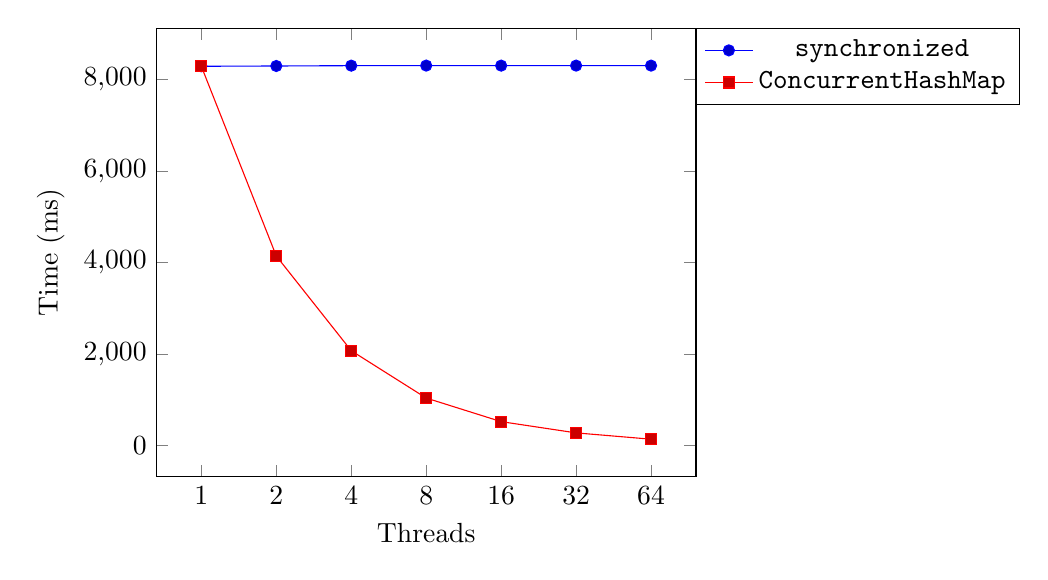
\begin{tikzpicture}
      \begin{axis}[
        % ybar,
        symbolic x coords={1,2,4,8,16,32,64},
        xtick=data,
        xlabel={Threads},
        ylabel={Time (ms)},
        legend style={at={(1.3,1)},anchor=north}
        ]
        \addplot coordinates {(1,8283.97) (2,8289.79) (4,8297.24) (8,8298.86) (16,8297.83) (32,8298.37) (64,8298.27)};
        \addplot coordinates {(1,8281.60) (2,4139.22) (4,2070.61) (8,1036.66) (16,521.31) (32,275.47) (64,137.65)};
        % \addplot coordinates {(1,17.45) (2,130.45) (4,210.27) (8,351.00) (16,749.40)};
        % \addplot coordinates {(1,8.28) (2,57.00) (4,126.49) (8,244.12) (16,486.06)};
        \legend{\texttt{synchronized}, \texttt{ConcurrentHashMap}}
      \end{axis}
    \end{tikzpicture}
  \end{center}
\end{frame}

% 1024 total, 8ms delay
% Benchmark: LocalCounter+Latch
% Local+Latch &  1 &     1024 & 8282.92 ms \
% Local+Latch &  2 &     1024 & 4139.20 ms \
% Local+Latch &  4 &     1024 & 2070.43 ms \
% Local+Latch &  8 &     1024 & 1036.67 ms \
% Local+Latch & 16 &     1024 & 519.34 ms \
% Local+Latch & 32 &     1024 & 262.71 ms \
% Local+Latch & 64 &     1024 & 138.20 ms \

% Benchmark: PerThreadMap+ConcurrentHashMap
% 1024
% PerThreadMap &  1 &     1024 & 8280.83 ms \
% 1024
% PerThreadMap &  2 &     1024 & 4140.86 ms \
% 1024
% PerThreadMap &  4 &     1024 & 2071.58 ms \
% 1024
% PerThreadMap &  8 &     1024 & 1037.81 ms \
% 1024
% PerThreadMap & 16 &     1024 & 521.22 ms \
% 1024
% PerThreadMap & 32 &     1024 & 271.26 ms \
% 1024
% PerThreadMap & 64 &     1024 & 138.21 ms \

\begin{frame}[fragile]
  \frametitle{Local Increment vs \texttt{ConcurrentHashMap} on 8ms}

  \begin{center}
    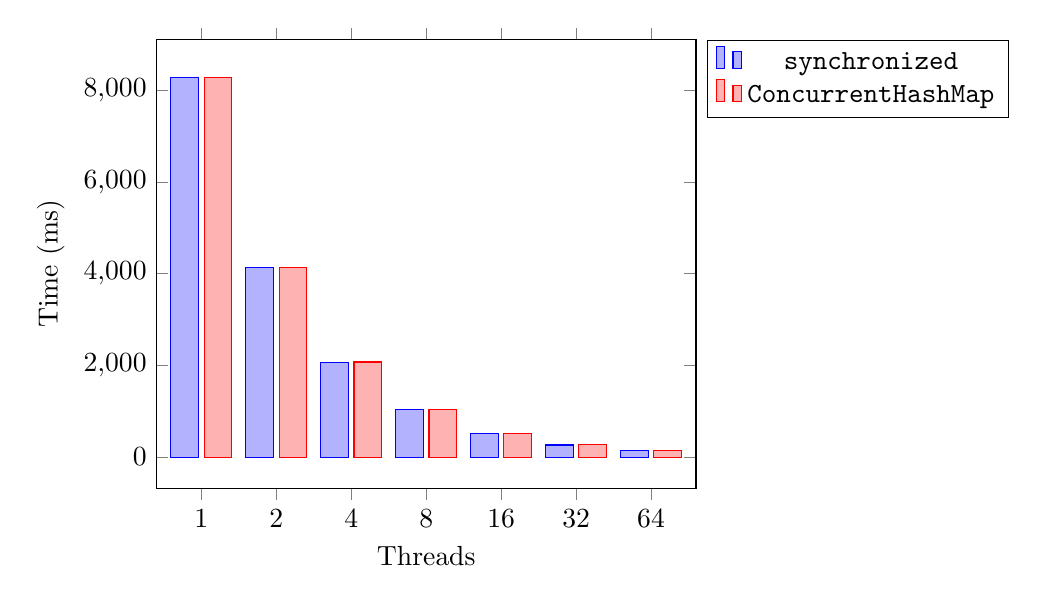
\begin{tikzpicture}
      \begin{axis}[
        ybar,
        symbolic x coords={1,2,4,8,16,32,64},
        xtick=data,
        xlabel={Threads},
        ylabel={Time (ms)},
        legend style={at={(1.3,1)},anchor=north}
        ]
        \addplot coordinates {(1,8282.92) (2,4139.20) (4,2070.43) (8,1036.67) (16,519.34) (32,262.71) (64,138.20)};
        \addplot coordinates {(1,8280.83) (2,4140.86) (4,2071.58) (8,1037.81) (16,521.22) (32,271.26) (64,138.21)};
        % \addplot coordinates {(1,17.45) (2,130.45) (4,210.27) (8,351.00) (16,749.40)};
        % \addplot coordinates {(1,8.28) (2,57.00) (4,126.49) (8,244.12) (16,486.06)};
        \legend{\texttt{synchronized}, \texttt{ConcurrentHashMap}}
      \end{axis}
    \end{tikzpicture}
  \end{center}
\end{frame}

\begin{frame}[fragile]
  \frametitle{Simple math}

  \begin{block}<1->{\faLightbulb \quad Key takeaway}
    The more computation intensive an independent task is, the more negligible
    the synchronization overhead is.
  \end{block}

  \vspace{0.4cm}

  \begin{block}<2->{\faLightbulb \quad Key takeaway}
    The larger the serialized part is, the less one stands to gain from parallelism.
  \end{block}

  \vspace{0.4cm}

  \begin{block}<3->{\faLightbulb \quad Amdahl's law}
    \[
      \mathrm{Speedup} \leq \frac{1}{F + \frac{1-F}{N}}
    \]
    In the above, $N$ is the number of threads and $F$ the \emph{fraction} of
    the \emph{serialized} code.
  \end{block}


\end{frame}

\begin{frame}[fragile]
  \frametitle{Last week's challenge}

  \begin{block}<1->{\faPuzzlePiece \quad Challege time!}
    Can someone come up with a multi-threaded/concurrency situation/problem setting
    where spinlocking, under circumstances, performs consistently and visibly
    better than \texttt{synchronized}? First three to demonstrate win half a point!
  \end{block}

  \vspace{0.4cm}

  \begin{block}<2->{\faLightbulb \quad Key takeaway}
    In this instance, we needed to make sure that enough synchronization attemps
    were made, but that the vast majority did not lock at all.
  \end{block}
\end{frame}

\begin{frame}[fragile]
  \Large{Moving on!}
\end{frame}

\begin{frame}[fragile]
  \frametitle{This week's topics}

  This week, we will look at...

  \begin{itemize}
  \item[\faBook]<1-> The \emph{producer-consumer} pattern.
  \item[\faBook]<1-> \texttt{Notify}-ing and \texttt{Wait}-ing.
  \item[\faBook]<1-> Task management with \texttt{BlockingQueue}'s.
  \item[\faBook]<1-> Task management with \texttt{Executor}'s.
  \end{itemize}
\end{frame}

\section{The producer-consumer pattern}

\begin{frame}[fragile]
  \frametitle{The producer-consumer pattern}

  \begin{block}<1->{\faLightbulb \quad Key idea}
    The \textbf{separation} of \emph{work to be done} from the \emph{execution}
    of the \emph{work}.
  \end{block}

  \begin{itemize}
  \item[\faBook]<1-> Presence of a data structure representing a to-do list.
    \begin{itemize}
    \item[\faBook]<1-> Producers identify work and create \emph{tasks} on the list.
    \item[\faBook]<1-> Consumers pick up (i.e. remove) tasks from the list and
      complete them.
    \end{itemize}
  \item[\faBook]<1-> Producers and consumers work independently.
  \end{itemize}

    \begin{block}<1->{\faPuzzlePiece \quad Key challenge}
      How do we pass work from producers to consumers safely and efficiently?
  \end{block}
\end{frame}

\begin{frame}[fragile]
  \frametitle{Examples of consumer-producer patterns}

  \begin{block}<1->{\faCookie \quad Kitchen}
    \begin{itemize}
    \item[\faBook] Waiter places orders on the board, the kitchen completes
      orders.
    \item[\faBook] Chefs put dishes on the counters, waiters must serve.
    \item[\faBook] Chefs produce tasks for each dish that the cooks must
      complete.
    \item[\faBook] Dish cleaning etc.
    \end{itemize}
  \end{block}
  \vspace{0.4cm}
  \begin{block}<2->{\faSearch \quad Factory}
    A certain line manufactures parts and consumers assemble the parts together.
  \end{block}
    \vspace{0.4cm}
  \begin{block}<3->{\faPrint \quad Printing}
    Users put printing jobs to the queue, printer picks jobs up and prints.
  \end{block}
\end{frame}

\begin{frame}[fragile]
  \frametitle{The pattern}

  \begin{table}[h]
    \centering
    \begin{tabularx}{\textwidth}{|l|X|}
      \hline
      \textbf{Role} & \textbf{Responsibility} \\
      \hline
      Producer & Generate data or tasks \\
      \hline
      Consumer & Process or act on them \\
      \hline
      Buffer & Temporarily stores work \\
      \hline
      Coordination & Ensures safe access and timing \\
      \hline
    \end{tabularx}
  \end{table}
\end{frame}

\begin{frame}[fragile]
  \frametitle{\faExclamationTriangle \quad Pitfalls}

  \begin{block}<1->{\faExclamationTriangle \quad No coordination}
    \begin{itemize}
    \item[\faUserInjured] Producers overwrite each other's items.
    \item[\faUserInjured] Consumers read nothing (or invalid data).
    \item[\faUserInjured] Threads spin or block forever (deadlock).
    \item[\faUserInjured] Shared buffer becomes corrupted.
    \end{itemize}
  \end{block}
  \vspace{0.4cm}
  \begin{block}<2->{\faBriefcaseMedical \quad Solution}
    We need a way to synchronize access to the buffer!
  \end{block}
\end{frame}

\begin{frame}[fragile]
  \frametitle{\faBriefcaseMedical \quad Solutions}

    \begin{table}[h]
    \centering
    \begin{tabularx}{\textwidth}{|l|X|}
      \hline
      \textbf{Approach} & \textbf{Tool} \\
      \hline
      Manual coordination	& \texttt{wait()}, \texttt{notify()} \\
      \hline
      Thread-safe buffer & \texttt{BlockingQueue} \\
      \hline
      Task abstraction & \texttt{ExecutorService}, queues \\
      \hline
      Fine-grained control & Semaphores, locks \\
      \hline
    \end{tabularx}
  \end{table}
\end{frame}

\begin{frame}[fragile]
  \frametitle{Busy-wait}

\begin{lstlisting}[language = Java , frame = trBL , firstnumber = last ,
escapeinside={(*@}{@*)}]
while ((something) == 0) {
        /* do nothing - just keep checking over and over */
    }

doSomething();
\end{lstlisting}

  \vspace{0.2cm}
  \begin{block}<1->{\faLightbulb \quad Key idea}
    Wait -- and keep checking -- until a condition is met.
  \end{block}
\end{frame}



\begin{frame}[fragile]
  \frametitle{Code Listings}

  \begin{itemize}
  \item[\faCode]<1-> LockTestHarness/Spinlock.java: Spinlock implementation
  \item[\faCode]<1-> LockTestHarness/LockTestHarness.java: Spinlock vs
    \texttt{synchronized} (single-run)
  \item[\faCode]<1-> LockTestHarness/LockTestHarness2.java: Spinlock vs
    \texttt{synchronized} (benchmark)
  \item[\faCode]<1-> LatchTestHarness/LatchTestHarness.java: Latch (local
    updates) vs
    \texttt{synchronized} (single)
  \item[\faCode]<1-> LatchTestHarness/LatchTestHarness2.java: Latch (local
    updates) vs
    \texttt{synchronized} (benchmark)
  \item[\faCode]<1-> LatchTestHarness/LatchTestHarness2Long.java: Proper
    benchmarking for latching and local updates using \texttt{long}'s.
  \item[\faCode]<1-> LatchTestHarness/LatchTestHarness2LongMap.java: Latch
    (local updates) vs \texttt{ConcurrentHashMap}.
  \end{itemize}

\end{frame}

\begin{frame}{}
  \centering \huge
  Thank you!
\end{frame}

\end{document}

%%% Local Variables:
%%% mode: latex
%%% TeX-engine: xetex
%%% TeX-master: t
%%% End:
